\section{Spec 2 --- Harmonised corpus}

All sources were mapped into one schema containing note, English translation, photo URLs, date, coordinates rounded to 1\,km,
country, water-body type, labels, licence, provenance, hashed user id. The language was identified with
lingua and notes were translated to English with OPUS-MT~\cite{tiedemann2020opusmt} and
NLLB-200~\cite{nllb2022}, with an automatic check for empty, looping, truncated and hallucinated output.
We masked personal names, e-mails and typed coordinates in notes.

\begin{table}[htbp]
\centering\small
\caption{Records per platform and modality (\%).}
\label{tab:platforms}
\resizebox{\columnwidth}{!}{%
\begin{tabular}{lrrrrl}
\toprule
Platform & Records & Text only & Image only & Both & Main languages \\
\midrule
iNaturalist & 85{,}899 & 4.3 & 76.9 & 18.7 & en \\
CrowdWater & 65{,}892 & 0.4 & 78.0 & 21.5 & en, de, et, es \\
Artportalen & 28{,}223 & 100 & 0 & 0 & sv \\
EyeOnWater & 26{,}758 & 0 & 100 & 0 & -- \\
Laji.fi & 16{,}707 & 100 & 0 & 0 & fi \\
Other GBIF & 1{,}670 & 100 & 0 & 0 & da \\
\midrule
Total & 225{,}149 & & & & 24 languages \\
\bottomrule
\end{tabular}}
\end{table}

Of the 80,886 notes, 32\% are Swedish, 25\% English, 16\% Finnish and 14\% undetermined. 
The other 20 languages are each under 5\% (Table~\ref{tab:platforms}). Figure~\ref{fig:waterbody} shows the
water-body type of the records per platform. Rivers and streams (36\%) come almost all from CrowdWater, lakes and
coasts from the Nordic portals and iNaturalist. Since EyeOnWater doesn't publish a locality type, a third is unknown.

\begin{figure}[htbp]
\centering
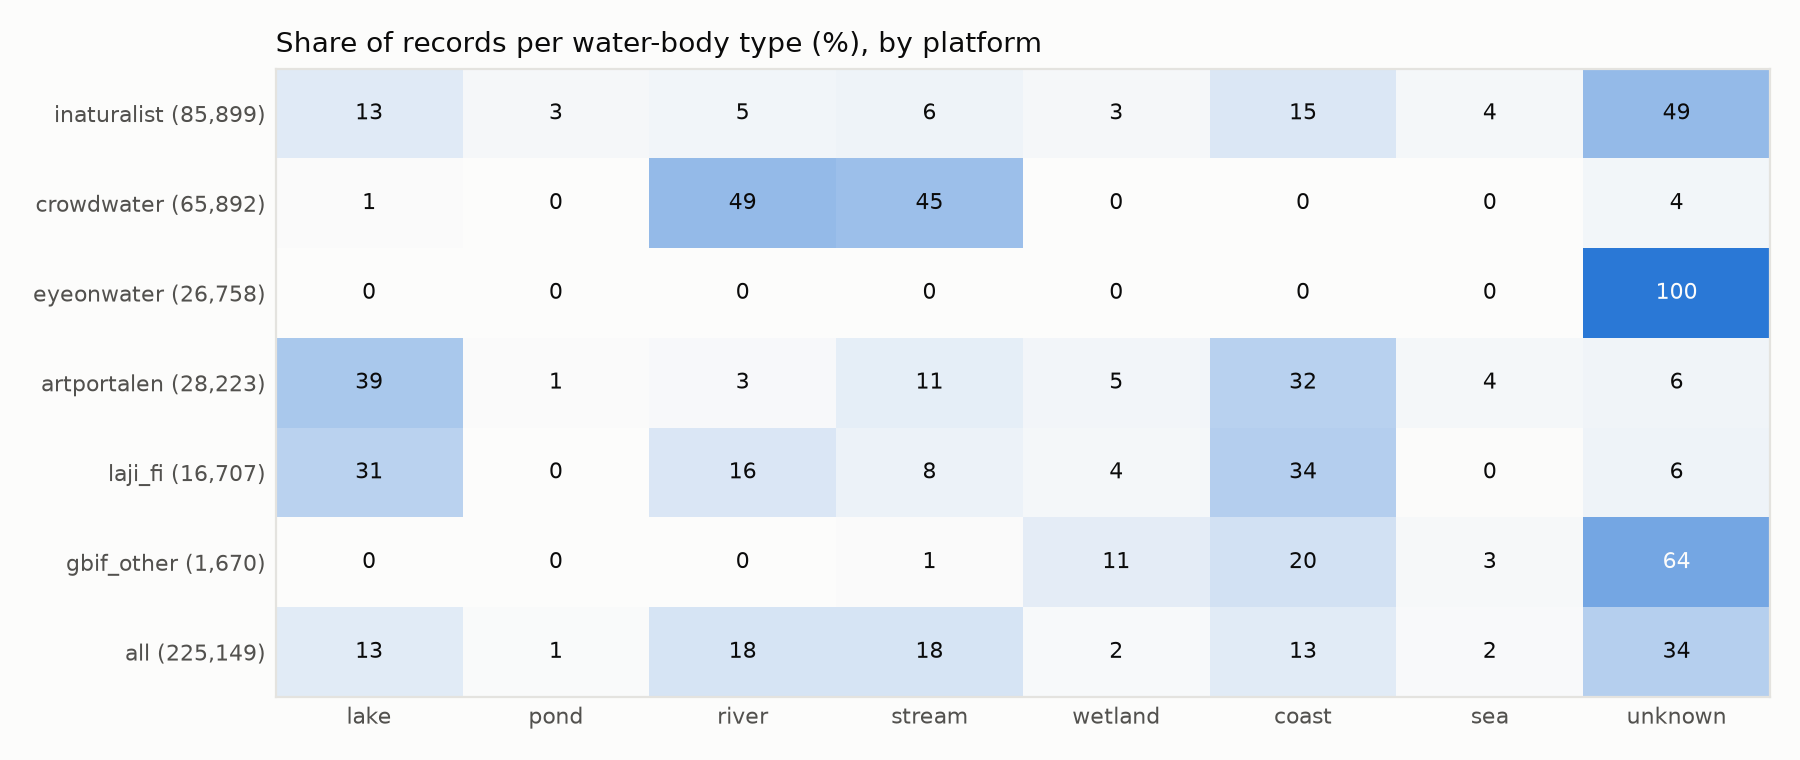
\includegraphics[width=\columnwidth]{stats_water_body_by_platform.png}
\caption{Share of records per water-body type and platform (\%).}
\label{fig:waterbody}
\end{figure}

\section{Spec 3 --- Corpus statistics}

Table~\ref{tab:corpus} compares the notes with the Brown~\cite{francis1979brown} and
Reuters-21578~\cite{lewis1997reuters} corpora. The notes are rather short, and many words are only seen once. Their higher
WordNet~\cite{miller1995wordnet} coverage comes from missing function words. FinnWordNet~\cite{linden2010finnwordnet}
covers 72\% of Finnish tokens.

\begin{table}[htbp]
\centering\small
\caption{Field notes vs edited text.}
\label{tab:corpus}
\resizebox{\columnwidth}{!}{%
\begin{tabular}{lrrr}
\toprule
 & Field notes & Brown & Reuters \\
\midrule
Mean length (tokens) & 3.2 -- 12.4 & 17.5 & 24.3 \\
Median length & 2 -- 7 & 15 & 23 \\
Words seen once & 49 -- 61\% & 43\% & 36\% \\
Types in 25k tokens & 4{,}622 -- 5{,}910 & 6{,}327 & 4{,}448 \\
Number tokens & 5 -- 15\% & 1\% & 10\% \\
WordNet coverage (English) & 76 -- 82\% & 70\% & 74\% \\
\bottomrule
\end{tabular}}
\end{table}

\section{Spec 4 --- Zipf and Heaps}

\textbf{Zipf}~\cite{zipf1949human}: OLS of log frequency on log rank, with the 90\% confidence interval of the slope,
$R^2$ and adjusted $R^2$ (Table~\ref{tab:zipf-platform}, Figure~\ref{fig:zipf}). The law holds ($R^2$ 0.95--0.98, like
Brown and Reuters).

\begin{table}[htbp]
\centering
\small
\caption{Zipf fits by platform (spec 4): OLS of $\log_{10}$ frequency on $\log_{10}$ rank with 90\% confidence interval of the slope.}
\label{tab:zipf-platform}
\resizebox{\linewidth}{!}{%
\begin{tabular}{lrrrrrrr}
\toprule
platform & types & slope & 90\% lo & 90\% hi & $R^2$ & adj. $R^2$ & slope top-1000 \\
\midrule
inaturalist & 16{,}209 & -1.289 & -1.292 & -1.287 & 0.973 & 0.973 & -0.952 \\
artportalen & 19{,}372 & -1.157 & -1.160 & -1.154 & 0.954 & 0.954 & -1.015 \\
crowdwater & 13{,}376 & -1.087 & -1.090 & -1.084 & 0.963 & 0.963 & -0.952 \\
laji\_fi & 9{,}511 & -0.972 & -0.976 & -0.968 & 0.950 & 0.950 & -0.949 \\
Brown & 47{,}039 & -1.323 & -1.325 & -1.321 & 0.974 & 0.974 & -0.977 \\
Reuters & 29{,}188 & -1.557 & -1.560 & -1.555 & 0.978 & 0.978 & -0.961 \\
\bottomrule
\end{tabular}
}
\end{table}


\begin{figure}[htbp]
\centering
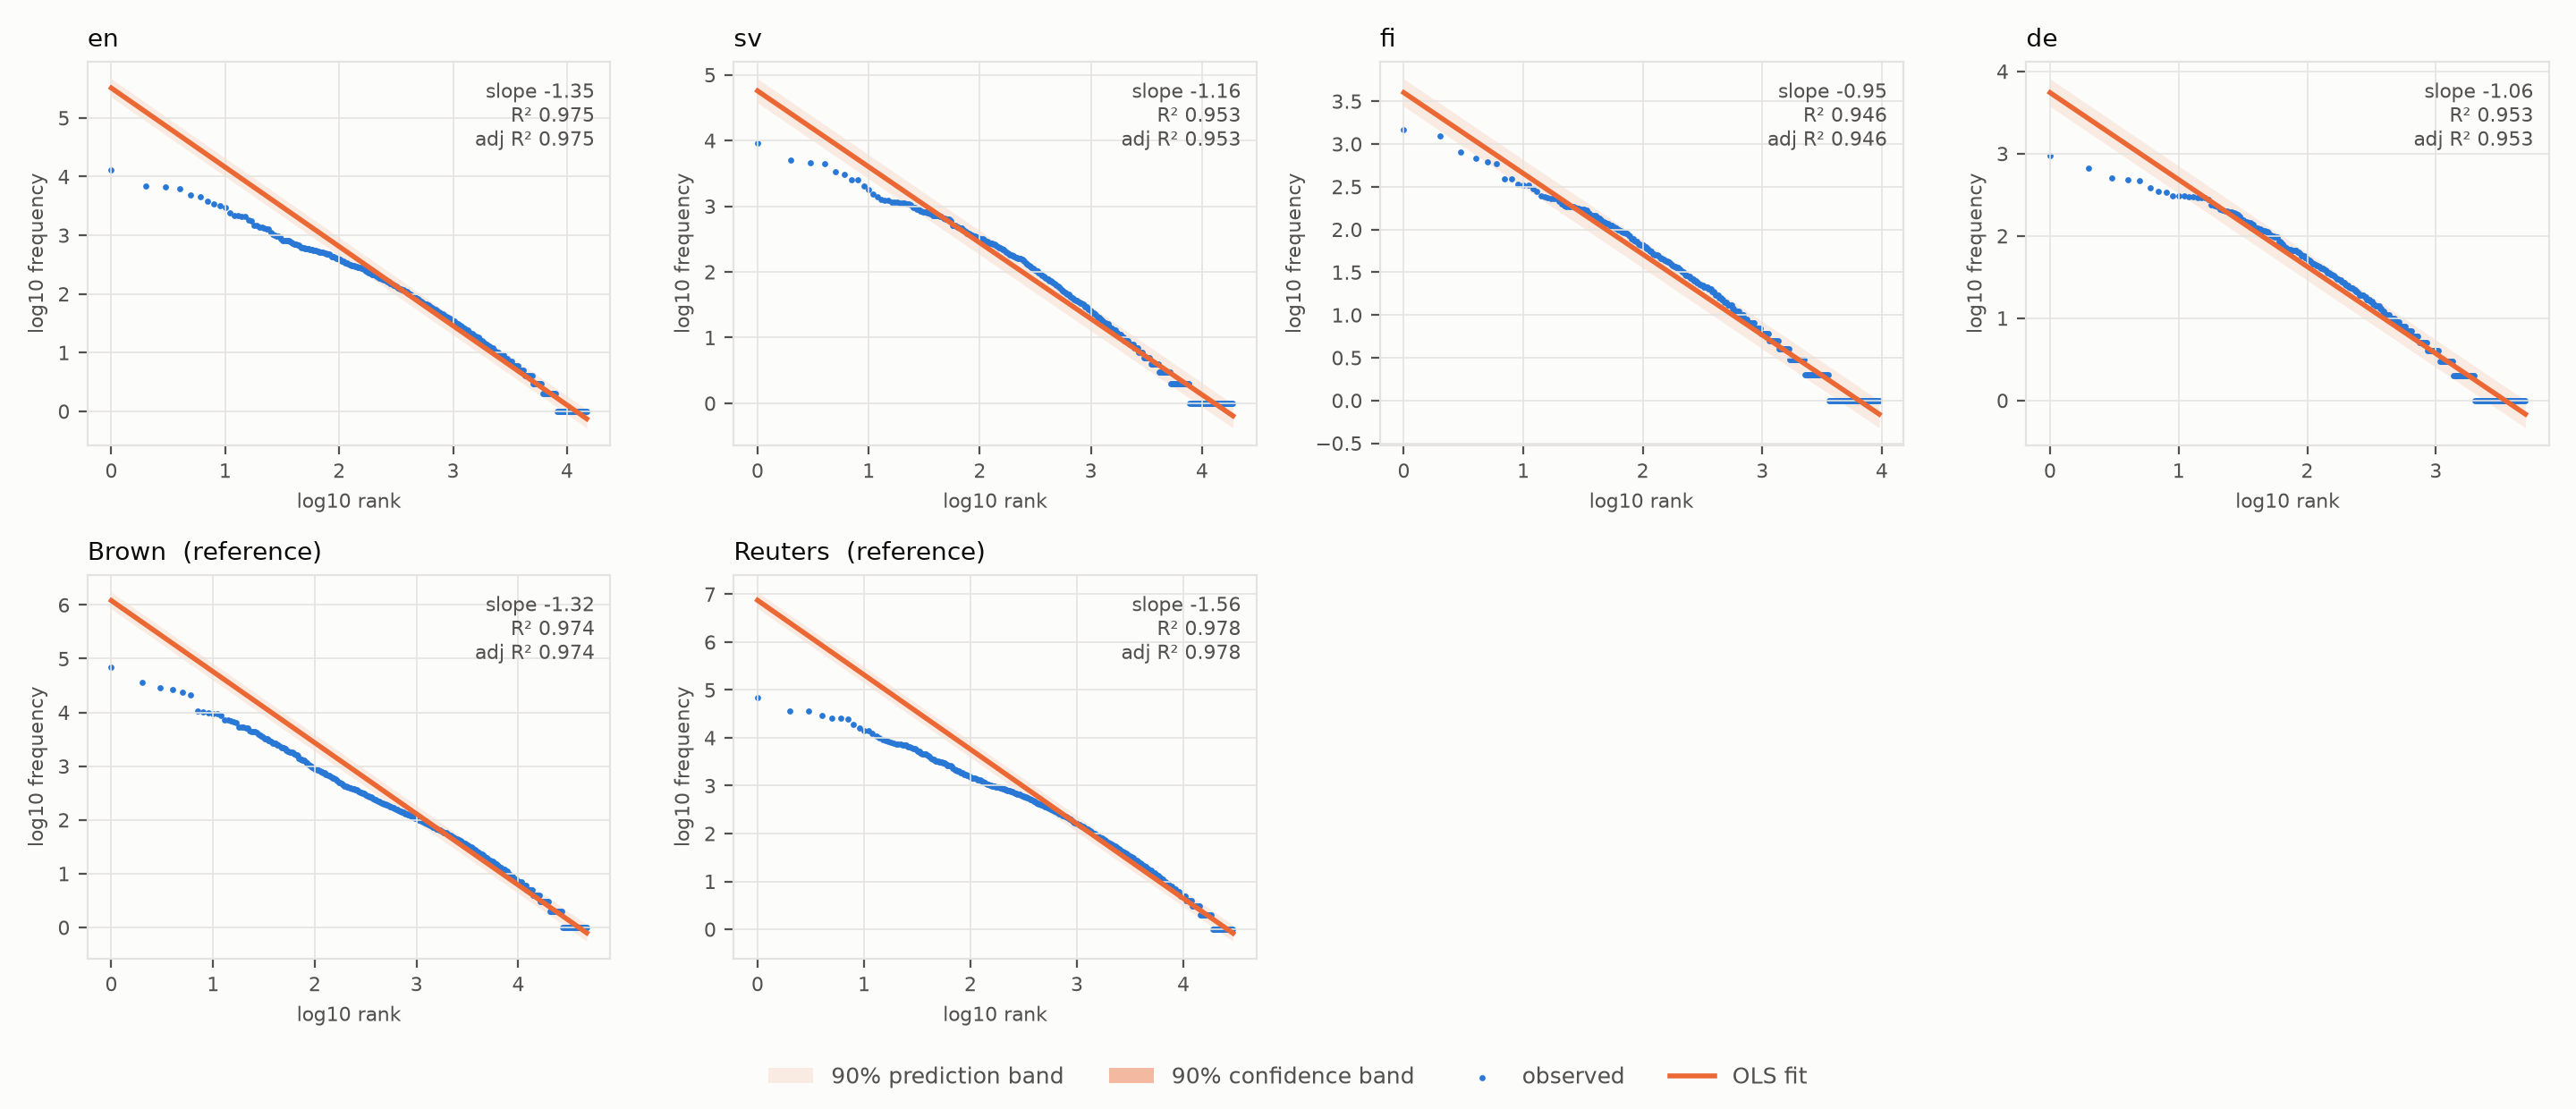
\includegraphics[width=\textwidth]{spec4_zipf_by_language.png}
\caption{Zipf plots by language with OLS fit, 90\% confidence band (dark) and 90\% prediction band (light).}
\label{fig:zipf}
\end{figure}

\textbf{Heaps}~\cite{heaps1978information}: vocabulary size $V$ at every 5\% of the tokens and is fitted as $V = K N^\beta$
(Table~\ref{tab:heaps-platform}, Figure~\ref{fig:heaps}). Here, the field notes grow faster ($\beta$ 0.55--0.68) than Brown
(0.51) and Reuters (0.45). 

\begin{table}[htbp]
\centering
\small
\caption{Heaps fits by platform (spec 4): $V = K N^\beta$ on vocabulary sizes at every 5\% of the tokens.}
\label{tab:heaps-platform}
\begin{tabular}{lrrrrrrr}
\toprule
platform & tokens & types & $K$ & $\textbackslash{}beta$ & 90\% lo & 90\% hi & $R^2$ \\
\midrule
inaturalist & 246{,}659 & 16{,}209 & 17.92 & 0.549 & 0.543 & 0.555 & 0.999 \\
artportalen & 224{,}669 & 19{,}372 & 8.71 & 0.626 & 0.623 & 0.629 & 1.000 \\
crowdwater & 103{,}315 & 13{,}376 & 10.37 & 0.622 & 0.616 & 0.628 & 1.000 \\
laji\_fi & 52{,}767 & 9{,}511 & 7.78 & 0.654 & 0.651 & 0.658 & 1.000 \\
Brown & 1{,}006{,}060 & 47{,}039 & 44.82 & 0.505 & 0.494 & 0.516 & 0.997 \\
Reuters & 1{,}330{,}267 & 29{,}188 & 55.22 & 0.446 & 0.439 & 0.454 & 0.998 \\
\bottomrule
\end{tabular}
\end{table}

\begin{table}[htbp]
\centering
\small
\caption{New word types added in selected 5\% steps of tokens, and the ratio of the last to the first step: growth slows down, much less for field notes than for edited text.}
\label{tab:heaps-inc}
\begin{tabular}{lrrrrrrr}
\toprule
 & 5\% & 10\% & 25\% & 50\% & 75\% & 100\% & last/first \\
\midrule
inaturalist & 3{,}065 & 1{,}520 & 870 & 596 & 442 & 415 & 0.14 \\
artportalen & 2{,}951 & 1{,}622 & 1{,}091 & 812 & 694 & 607 & 0.21 \\
crowdwater & 2{,}075 & 1{,}212 & 818 & 610 & 449 & 358 & 0.17 \\
laji\_fi & 1{,}326 & 786 & 496 & 378 & 332 & 332 & 0.25 \\
Brown & 9{,}939 & 5{,}227 & 2{,}668 & 1{,}709 & 1{,}292 & 1{,}023 & 0.10 \\
Reuters & 7{,}508 & 3{,}143 & 1{,}621 & 952 & 750 & 548 & 0.07 \\
\bottomrule
\end{tabular}
\end{table}


\begin{figure}[htbp]
\centering
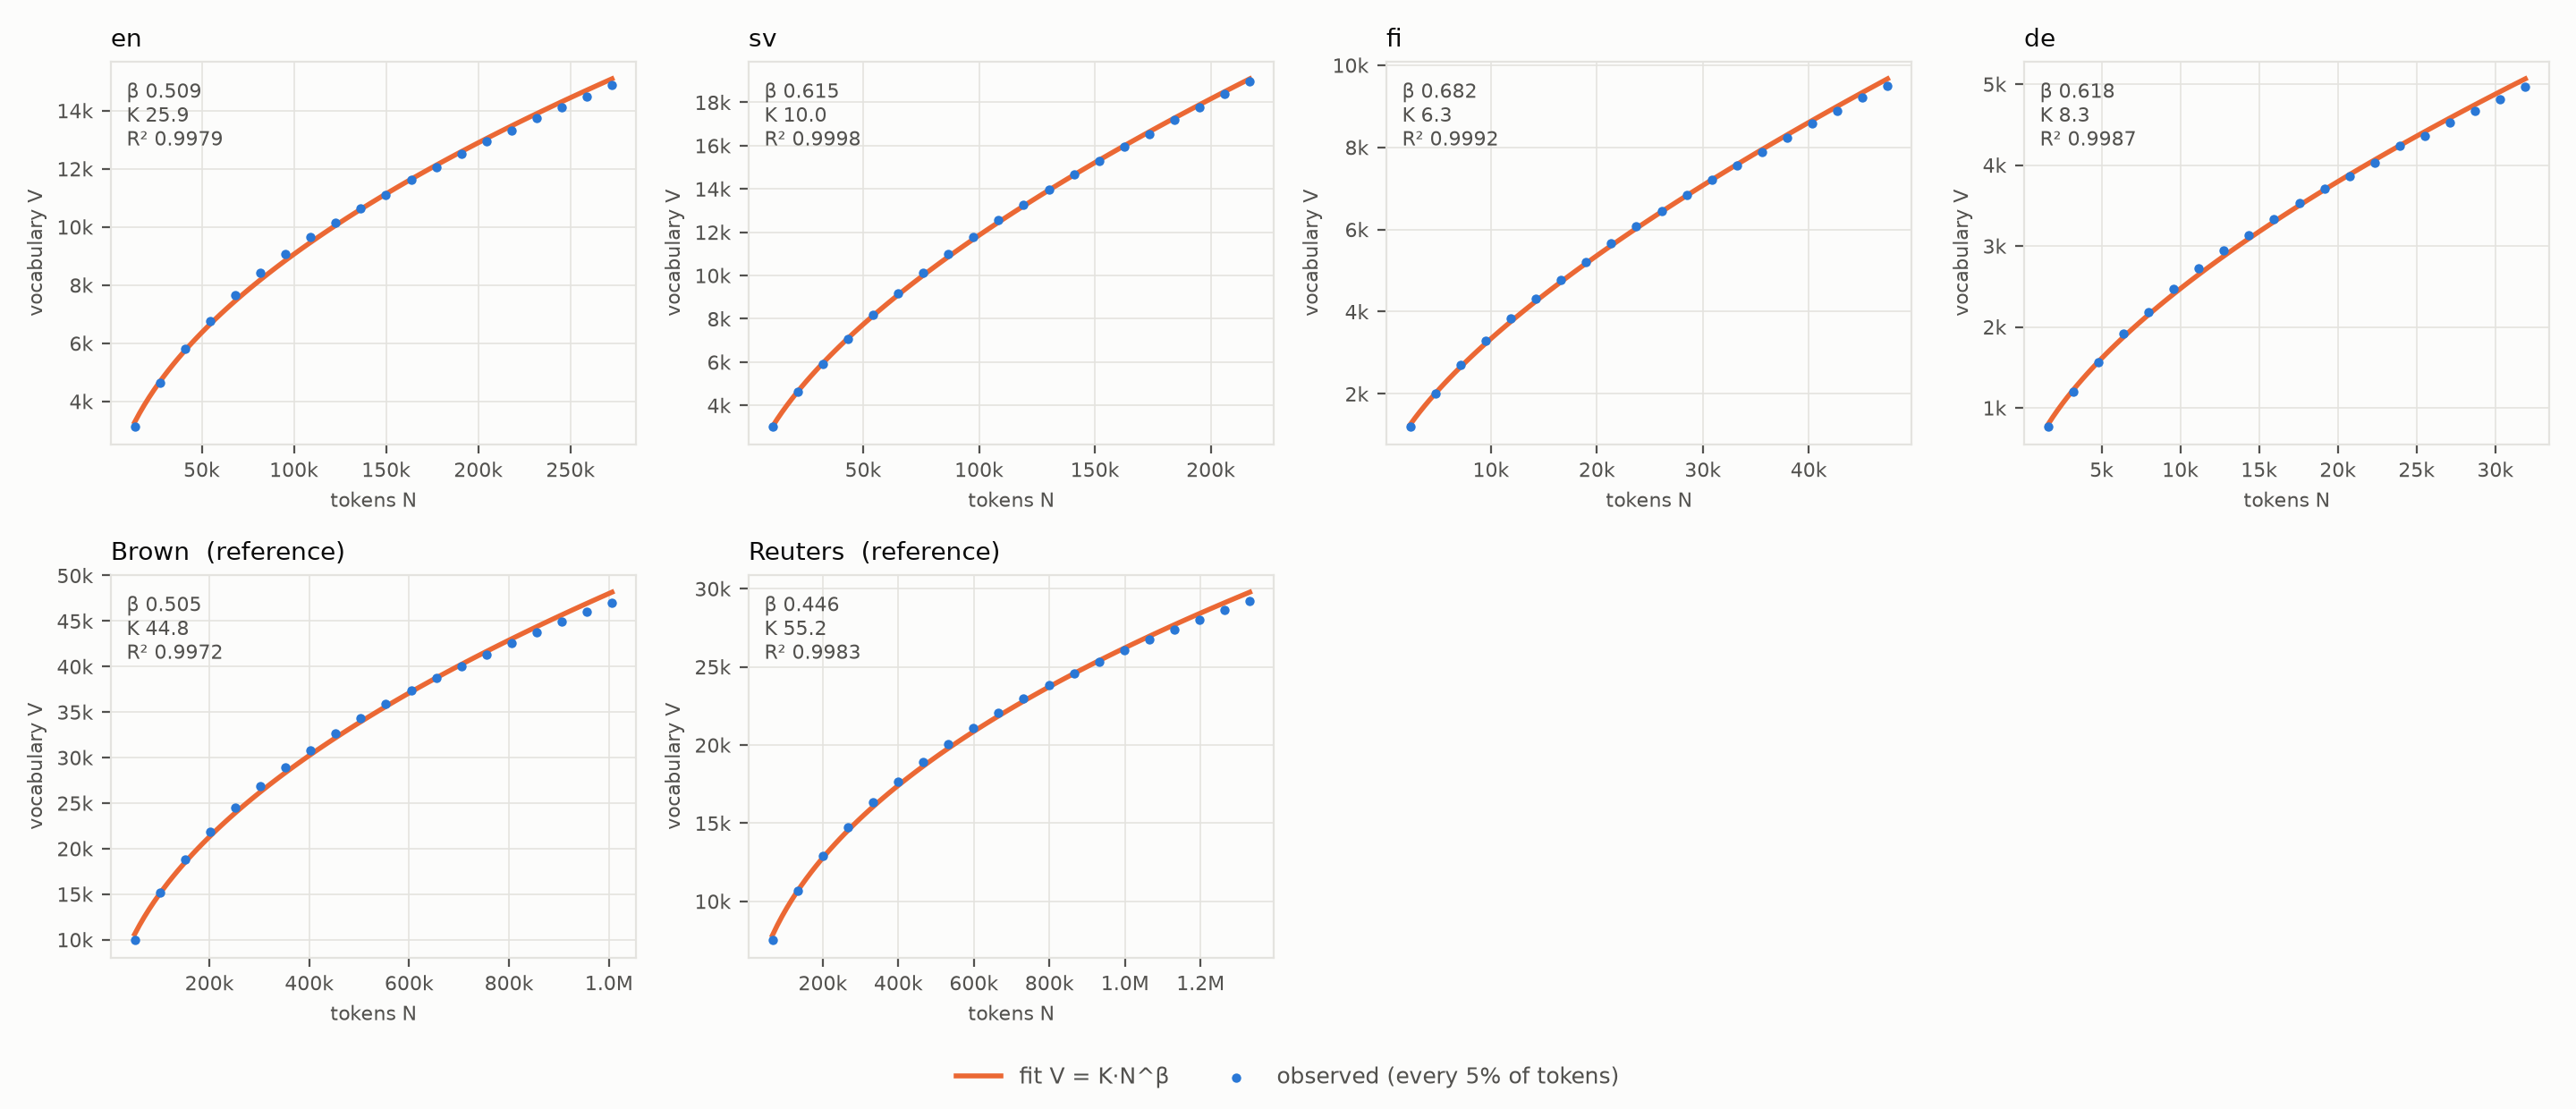
\includegraphics[width=0.78\textwidth]{spec4_heaps_by_language.png}
\caption{Heaps curves by language: vocabulary size against tokens, with fitted $V = K N^\beta$.}
\label{fig:heaps}
\end{figure}
